
% !TeX spellcheck = en_US

\chapter{Introduction to Flyway}


\section{Overview}
\marginpar{Information}%
Flyway is a tool that makes database migrations easy and provides version control for databases. It is a multi-platform and cross-database tool with support for over 20 databases.
Axel Fontaine from Google Code created Flyway in 2010 and was acquired by Redgate Software in 2019. Flyway is currently at the 9th version when creating this work. The creator was looking for a simple method to implement database changes quickly and directly in \gls{SQLg}. His main goal was to include database changes as part of the software deployment process \cite{Robles2021}.
Flyway uses the freemium business model. The basic version is free and open source \cite{Fontaine2010} and additionally, there is a paid Teams or Enterprise Edition available.

With Flyway, migration files are written in either with \gls{SQLg} (database-specific syntax (such as PL/SQL, T-SQL) or \gls{JAVAg} (for advanced data transformations or dealing with LOBs). Flyway can connect to databases hosted in on-premises or cloud environments, thanks to the included JDBC driver library that is shipped with the tool. It runs on all modern platforms, such as Linux, Mac or Windows.  \cite{Dillon2022} \cite{DBMSTools}


\marginpar{Migrations \cite{Parsick2018} \cite{Lukonin2017}}%
There are four possibilities of migrations as shown in \autoref{tab:migration_types}. There are versioned migrations with scripts with a unique meanings, executed only once. These versioned migrations are mainly used for Data Definition Language (DDL), like creating or modifying a table.

Repeatable migration scripts do not have a version number. These are always if their checksum changes and after the versioned migrations are applied. Typical applications for repeatable tasks are importing base data, rebuilding views or indexes, and adding permissions or other maintenance tasks.

\begin{table}[h]
	\centering
	\begin{tabularx}{8cm}{X c c}
		Basis & Versioned & Repeatable \\ \toprule
		SQL based & \checkmark & \checkmark \\
		Java based & \checkmark & \checkmark \\
	\end{tabularx}
	\caption{Migration Types - Based on Parsick et al. \cite{Parsick2018}}
	\label{tab:migration_types}
\end{table}

\marginpar{SQL Migrations}%
Flyway developers can migrate changes directly with \gls{SQLg}. Per default, Flyway takes the database migrations from the directory \textit{sql}.
These \gls{SQLg} migration files have to follow the naming convention:

\begin{center}
\begin{tabularx}{8cm}{r l}
Versioned & \texttt{\textcolor{blue}{V}\textcolor{green}{1\_1\_1}\textcolor{red}{\_\_}\textcolor{orange}{create\_table}.sql}\\
Repeatable & \texttt{\textcolor{blue}{R}\textcolor{red}{\_\_}\textcolor{orange}{create\_table}.sql}\\
\end{tabularx}
\end{center}

\begin{flushright}
\textcolor{blue}{Prefix}\\
\textcolor{green}{Version}\\
\textcolor{red}{Seperator (two underscores)}\\
\textcolor{orange}{Description}\\
\end{flushright}

\todo{Table and Legend are ugly.}

These \gls{SQL} scripts can have several rows and allow all database-specific syntax, including comments. These \gls{SQL} migrations are mainly used for DDL changes such as create, alter, and drop for simple data changes.

\marginpar{Java Migrations}%
Unlike changes in \gls{SQL}, \gls{JAVAg} changes are more for BLOB or CLOB changes or for progressive changes to an extensive data set like recalculations. The naming convention is similar; only the ending differs.

\todo{Add BLOB, CLOB to glossary.}

\begin{center}
	\begin{tabularx}{8cm}{r l}
		Versioned & \texttt{\textcolor{blue}{V}\textcolor{green}{1\_1\_1}\textcolor{red}{\_\_}\textcolor{orange}{create\_table}.java}\\
		Repeatable & \texttt{\textcolor{blue}{R}\textcolor{red}{\_\_}\textcolor{orange}{create\_table}.java}\\
	\end{tabularx}
\end{center}

\marginpar{Advanced Changes\\ \cite{Parsick2018}}%
Some migration steps need user intervention, for example, creating a materialized view. This functionality is provided by flyway with callback functions. 

\begin{figure}[H]
	\centering
	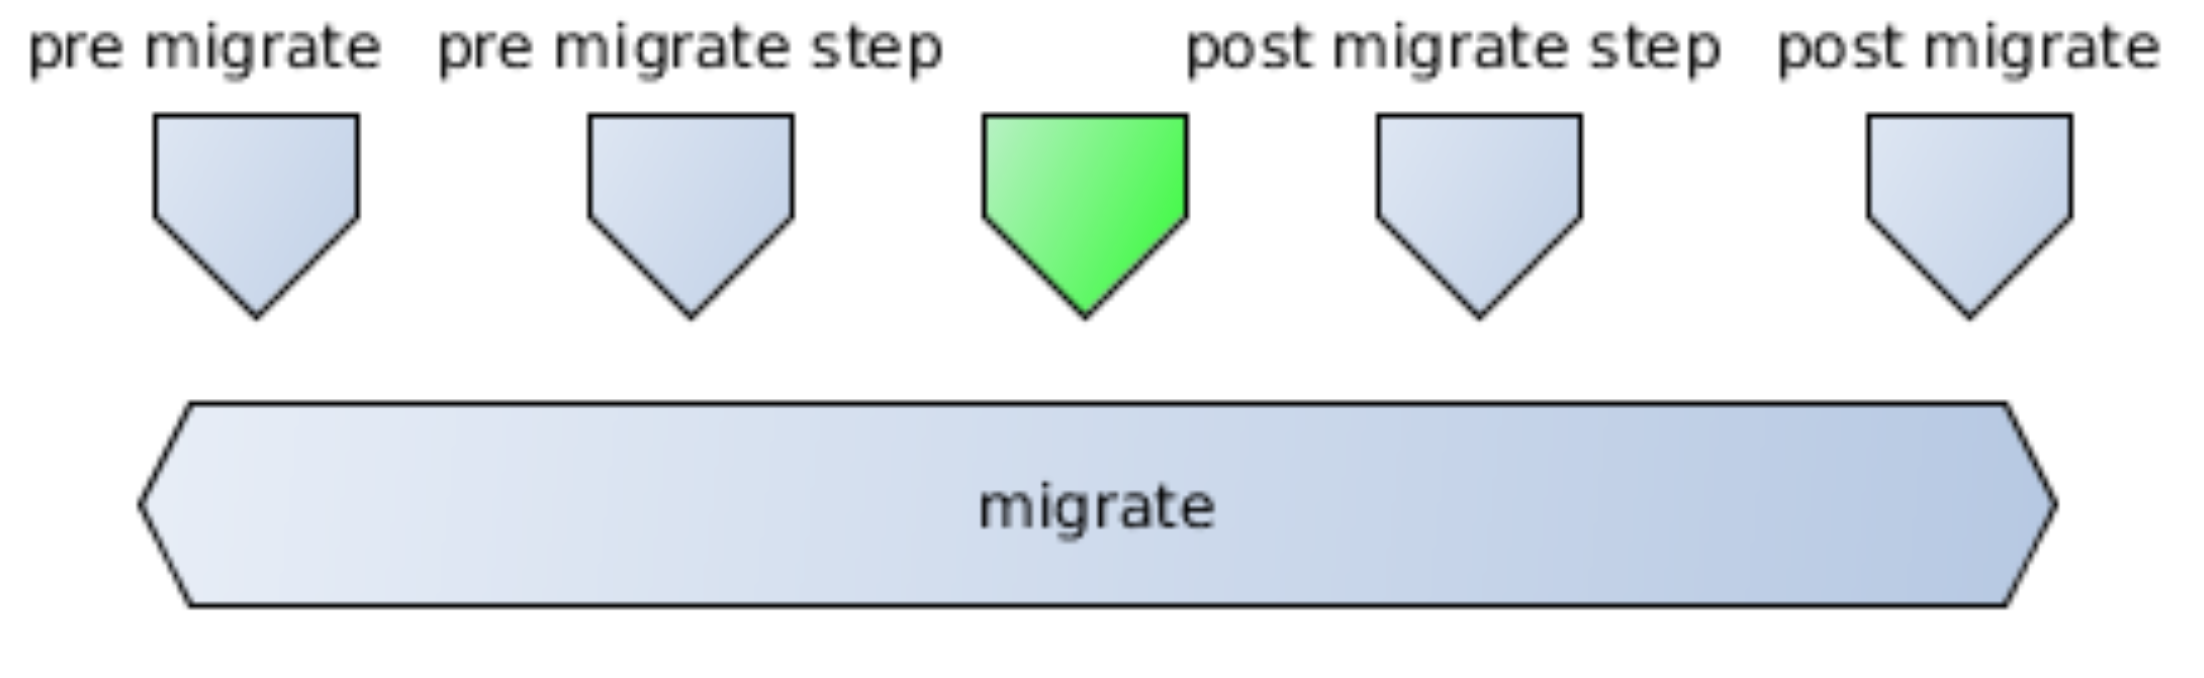
\includegraphics[width=0.6\textwidth]{./chapters/intro_flyway/images/advanced_migrations}
	\caption[Flyway Lifecycle - Source: \cite{Parsick2018}]{Flyway Lifecycle}
	\label{fig:advanced_migrations}
\end{figure}

There are several options for the execution times. The defined naming convention recognizes these times. The callbacks can be written in \gls{SQLg} or \gls{JAVAg}. 

\begin{lstlisting}[caption=SQL Callback Functions for Flyway - Source: \cite{FlywayCallbacks}]
BeforeMigrate.sql
BeforeEachMigrate.sql
AfterEachMigrate.sql
AfterMigrate.sql
\end{lstlisting}

If the task needs to be more powerful or flexible, \gls{JAVAg} callbacks can be formulated as follows:
\begin{lstlisting}[caption=Java Callback Functions before clean - Source: \cite{FlywayCallbacks}]
public interface FlywayCallback {
	/**
	* Runs before the tasks executes
	* by avoiding unnecessary connection state setups for events 
	* that will not be handled anyway.
	* @param valid connection to a database
	*/
	void beforeClean(Connection connection);
}
\end{lstlisting}
Other callback function can be formulated with the same name as the SQL-functions.

\marginpar{Dealing with Hotfixes\\ \cite{Lukonin2017}}%
To apply Flyway migrations out of order and fill in any gaps, activate the \textit{outOfOrder} property. This functionality is useful when the production environment is older, but the development and test environments are already at a new version. Hotfixes in between can then be applied by activating the \textit{outOfOrder} property. In addition, as described in the introduction \autoref{best_practices}, if you have multiple developers working on different branches, it may be helpful to enable the \textit{outOfOrder} property to allow for more flexibility in the migration and branching process.


\marginpar{Flyway Teams \cite{FlywayTeams}}%
The Pro-Version of Flyway is called Flyway Teams. This pro version costs (as of creation of this work) 447€ per user per year. It offers:
\begin{itemize}
	\item Additional migration controls
	\item Protect against failed deployments
	\item Professional technical support from Redgate
	\item Support for older DB versions
	\item Built-in Git client and object-level versioning
\end{itemize}

Compared to the team version, the free, open-source version includes the core functionalities with desktop \gls{GUI} support for only the current database versions and support through the community. The core functionalities include the six basic commands: migrate, clean, info, validate, baseline and repair.

A comparison between the Flyway editions can be found here \autoref{label}.\\
\todo{Liste einfügen in Anhang}

\marginpar{Community}%
Stars on GitHub: 6'900 (27. December 2022)\\
Tags on StackOverflow: 2,118 (31. December 2022)\\

\marginpar{Learning\\ Materials}%
Please refer to the following sources to get started with Flyway:
\todo{List of Links? maybe add cite?}
\begin{itemize}
	\item \href{https://www.red-gate.com/hub/university/courses/flyway}{Redgate University Flyway training courses}
	\item \href{https://flywaydb.org/documentation}{Get Started Documentation}
	\item \href{https://www.youtube.com/playlist?list=PLhFdCK734P8DYHYYWaJpzJJ-qZFZ_JTHM}{Redgate Youtube Channel}
	\item \href{https://www.youtube.com/watch?v=dzRzlDpdDW4}{Flyway talk by Sandra Parsick}
\end{itemize}

\section{Features \label{flyway_features}}
Below are some of the most useful Flyway commands are presented:


\textbf{Info}\\
Get an overview of the applied migrations and their success status.\\

\begin{figure}[H]
	\centering
	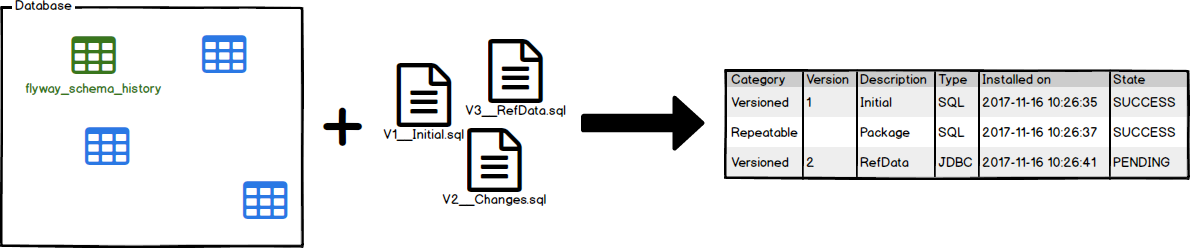
\includegraphics[width=0.8\textwidth]{./chapters/intro_flyway/images/command-info}
	\caption[Flyway Info - Source: \cite{FlywayGetStarted}]{Flyway Info}
	\label{fig:command-info}
\end{figure}

\todo{write all titles big or small?}
\textbf{clean}\\
With \texttt{flyway clean}, one can drop all objects, like tables, views and triggers, in the configured schemas. It serves as a reset but is dangerous in a production environment.

\textbf{Validate}\\
To ensure that all migrations are applied correctly,  \texttt{flyway validate} is the choice command. The validation checks if the migration locally has the same checksum as the migration executed in the database.
There is a possibility to apply custom validation rules. Because in a productive environment, there will be hotfixes, deleted migrations and other changes that break the default validation conventions. Custom rules are only available in the teams edition.

\textbf{Repair}\\
However, if something is broken, the repair command can repair the database, especially the checksum. For example, when a database migration fails, the migration is marked as failed in the schema history table (\textit{flyway\_schema\_history}). However, if a database supports \gls{DDL} transactions (like PostgreSQL), the failed migration is rolled back automatically, and nothing is recorded in the schema history table. Nevertheless, if the database does not support DDL transactions (e.g. Oracle Database, MySQL, MariaDB), you have two options to repair the database and remove the failed entries:

\begin{enumerate}
	\item Run \texttt{flyway repair}\\
	\item One uses the flyway callback functions. One could use the \textit{afterMigrateError} and add a SQL-script to this callback, which deletes the failed migration entry in the \textit{flyway\_schema\_history} table.
	
	\begin{lstlisting}[language=SQL]
		DELETE IGNORE FROM flyway_schema_history WHERE success=0;
	\end{lstlisting}
\end{enumerate}


\textbf{Undo}\\
To undo the most recent migration applied to the database, run \texttt{flyway undo}. The undo command can be repeated until the database is converted back to version 1. Undo assumes that the previously applied migration succeeded and now should be undone. If the previously applied migration fails, repair the migrations before applying the undo command. The undo command is a Teams Edition feature only.

\textbf{Baseline}\\
This command makes the current database the baseline for the future. This will cause the migrate command to ignore all migrations up to the actual version. This can be useful to reduce the overhead if many old migrations scripts exist that will not be used again.

\section{Installation and Setup}
\marginpar{Different usages of Flyway \cite{FlywayGetStarted}}%
Flyway can be used with the following programs or tools.

\begin{minipage}[t]{0.5\textwidth}
\textbf{Flyway Clients}

\begin{itemize}
	\item \Gls{CLI}
	\item \gls{JAVAg} \acrshort{API}
	\item Maven
	\item Gradle
\end{itemize}
\end{minipage}
\begin{minipage}[t]{0.5\textwidth}
	\textbf{Third Party Plugins}
	\begin{itemize}
		\item Jenkins
		\item IntelliJ IDEA
		\item NPM
		\item Play
		\item Spring Boot
		\item etc.
	\end{itemize}
\end{minipage}
\vspace{0.3cm}

\marginpar{CLI installation}%
Download the latest version of the \href{https://flywaydb.org/download/community}{Flyway Cummunity Edition} and extract the downloaded file. To execute the flyway commands, one need a java installation.
Once extracted, the file becomes a directory with the following structure:

\begin{figure}[H]
    \centering
    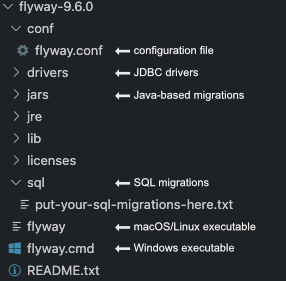
\includegraphics[width=0.4\textwidth]{./chapters/intro_flyway/images/flyway_folder_structure}
   \caption[Flyway folder structure - Source: Own illustration]{Flyway folder structure}
    \label{fig:flyway_folder_structure}
\end{figure}


\marginpar{Configuration}%
To connect to a running database, add the relevant information to \textit{conf/flyway.conf}.
In our minimal example this could be:

\begin{lstlisting}[caption=Minimal configuration]
flyway.url=jdbc:postgresql://localhost:5432/pagila
flyway.user=postgres
flyway.password=password
\end{lstlisting}

This is just a minimal configuration, but there are many more additional parameters that can be set \footnote{\url{https://flywaydb.org/documentation/configuration/parameters/}}.


\marginpar{Workaround Mac OS}%
To make the flayway command know on MacOS:
\begin{lstlisting}[caption=Minimal configuration]
export PATH=$PATH:/Users/marco/Documents/DB-Seminar/flyway-9.8.1
\end{lstlisting}
Running a flyway command for the first time, the error message \textit{„java“ kann nicht geöffnet werden, da der Entwickler nicht verifiziert werden kann.} occurs. Go to Security in settings and allow the java instance to run.

\newpage